%------------------------------------------------------------------------------
%	ARARA DIRECTIVES
%------------------------------------------------------------------------------

% arara: clean: { files: [arara.log, main.aux, main.bbl, main.bcf, main.blg, main.idx, main.ilg, main.ind, main.log, main.nav, main.out, main.ptc, main.run.xml, main.synctex.gz, main.snm, main.toc, main.vrb] }

% arara: xelatex: { synctex: yes, options: "-halt-on-error -file-line-error-style", shell: yes}
% arara: bibtex
% arara: xelatex: { options: "-halt-on-error -file-line-error-style", shell: yes}
% arara: xelatex: { synctex: yes, options: "-halt-on-error -file-line-error-style", shell: yes}

%------------------------------------------------------------------------------

\documentclass[xcolor={svgnames}]{beamer}

% This file is a solution template for:

% - Talk at a conference/colloquium.
% - Talk length is about 20min.
% - Style is ornate.

% Copyright 2004 by Till Tantau <tantau@users.sourceforge.net>.
%
% In principle, this file can be redistributed and/or modified under
% the terms of the GNU Public License, version 2.
%
% However, this file is supposed to be a template to be modified
% for your own needs. For this reason, if you use this file as a
% template and not specifically distribute it as part of a another
% package/program, I grant the extra permission to freely copy and
% modify this file as you see fit and even to delete this copyright
% notice.


\mode<presentation>
{
  % \usetheme{Warsaw}
  % or ...
  \usetheme{Boadilla}
  \useoutertheme{miniframes}
  \useinnertheme{circles}

  \setbeamercovered{transparent}
  % or whatever (possibly just delete it)

  % \setbeamercolor{palette primary}{bg=dblpBlue,fg=dblpYellow}
  % \setbeamercolor{palette secondary}{bg=dblpYellow,fg=dblpBlue}
  % \setbeamercolor{palette tertiary}{bg=THOrange,fg=white}
  % \setbeamercolor{palette quaternary}{bg=THRed,fg=white}
  % \setbeamercolor{structure}{fg=dblpBlue} % itemize, enumerate, etc
  % %\setbeamercolor{section in toc}{bg=THRed, fg=white} % TOC sections
  %
  % \setbeamercolor{title}{fg=dblpYellow}
  % \setbeamercolor{frametitle}{fg=dblpYellow}
  %
  % \setbeamercolor{section in head/foot}{fg=white, bg=dblpYellow}
}

%for notes during presentation
\usepackage{pgfpages}
\setbeameroption{show notes on second screen}

% workaround for bug with notes + xelatex, see https://github.com/josephwright/beamer/issues/337
\makeatletter
\def\beamer@framenotesbegin{% at beginning of slide
     \usebeamercolor[fg]{normal text}
      \gdef\beamer@noteitems{}%
      \gdef\beamer@notes{}%
}
\makeatother

\usepackage{my-beamer} %custom beamer template
\usepackage{lmodern}

\usepackage[svgnames]{xcolor}
\usepackage{my-xcolor} % custom colors
\usepackage{xcolor-material}

\usepackage{fontspec} %custom fonts
\setmainfont{Roboto Light}
\setsansfont{Roboto Light}
\setbeamerfont{footnote}{size=\tiny}

\usepackage[english]{babel}
% or whatever

% \usepackage[latin1]{inputenc}
% or whatever

\usepackage{times}
\usepackage[T1]{fontenc}
% Or whatever. Note that the encoding and the font should match. If T1
% does not look nice, try deleting the line with the fontenc.

\usepackage{booktabs} % For formal tables
\usepackage{csvsimple} %input tables from csv
\usepackage{threeparttable}

\usepackage{mathtools} % cases for math
\usepackage{amsmath}

\usepackage{xspace}

\usepackage{nameref}
\makeatletter
\newcommand*{\currentname}{\@currentlabelname}
\makeatother

\newcommand{\ndcg}[1]{\ensuremath{\textsf{ndcg}\textsf{#1}}\xspace}

\usepackage{tikz} %frontend to the pgf system
\usetikzlibrary{calendar, shapes.geometric}
\usetikzlibrary{calc}

\usepackage[beamer,customcolors]{hf-tikz}

\tikzset{hl/.style={
    set fill color=red!80!black!40,
    set border color=red!80!black,
  },
}
\RenewDocumentCommand{\tikzmarkin}{r<> o m D(){\belowrightoff} D(){\aboveleftoff}}{%
  \IfNoValueTF{#2}{%true-val
    \only<#1>{\tikz[remember picture,overlay]
      \draw[line width=1pt,rectangle,disable rounded corners,fill=\fcol,draw=\bcol]
      (pic cs:#3) ++(#4) rectangle (#5) node [anchor=base] (#3){}
      ;}%
  }{%false-val
    \only<#1>{\tikz[remember picture,overlay]
      \draw[line width=1pt,rectangle,disable rounded corners,fill=\fcol,draw=\bcol,#2]
      (pic cs:#3) ++(#4) rectangle (#5) node [anchor=base] (#3){}
      ;}}%
}

\usepackage[backend=bibtex,firstinits=true]{biblatex}
\bibliography{main}
\AtEveryCitekey{%
\clearfield{url}%
\clearfield{doi}%
\clearfield{isbn}%
\clearfield{pages}%
\clearfield{series}%
}

%------------------------------------------------------------------------------

\title[Prioritizing Conferences for Harvesting] % (optional, use only with long paper titles)
{Prioritizing and Scheduling Conferences for Metadata Harvesting in dblp}

\author[Mandy Neumann] % (optional, use only with lots of authors)
{\underline{M.~Neumann\inst{1}} \and C.~Michels\inst{2} \and P.~Schaer\inst{1} \and R.~Schenkel\inst{2}}
% - Give the names in the same order as the appear in the paper.
% - Use the \inst{?} command only if the authors have different
%   affiliation.

\institute[TH K\"oln] % (optional, but mostly needed)
{
  \inst{1}%
  Department of Information Science\\
  TH K\"oln (University of Applied Sciences)
  \and
  \inst{2}%
  Department of Computer Science\\
  University of Trier}
% - Use the \inst command only if there are several affiliations.
% - Keep it simple, no one is interested in your street address.

\date[LWDA 2019] % (optional, should be abbreviation of conference name)
{Lernen. Wissen. Daten. Analysen. LWDA 2019}
% - Either use conference name or its abbreviation.
% - Not really informative to the audience, more for people (including
%   yourself) who are reading the slides online

\subject{Digital Libraries}
% This is only inserted into the PDF information catalog. Can be left
% out.


% If you have a file called "university-logo-filename.xxx", where xxx
% is a graphic format that can be processed by latex or pdflatex,
% resp., then you can add a logo as follows:

\pgfdeclareimage[height=0.5cm]{university-logo}{img/dblp.logo.320x120.eps}
\logo{\pgfuseimage{university-logo}}



% Delete this, if you do not want the table of contents to pop up at
% the beginning of each subsection:
% \AtBeginSubsection[]
% {
%   \begin{frame}<beamer>{Outline}
%     \tableofcontents[currentsection,currentsubsection]
%   \end{frame}
% }


% If you wish to uncover everything in a step-wise fashion, uncomment
% the following command:

%\beamerdefaultoverlayspecification{<+->}

%------------------------------------------------------------------------------
%------------------------------------------------------------------------------
\begin{document}

\begin{frame}[plain]
  \titlepage
\end{frame}

\begin{frame}{Outline}
  \tableofcontents[subsectionstyle=hide]
  % You might wish to add the option [pausesections]
\end{frame}

\AtBeginSection[] {
  \begin{frame}{Outline}
  	\tableofcontents[
      currentsection,
      currentsubsection,
      subsectionstyle=hide
    ]
  \end{frame}
}
%------------------------------------------------------------------------------
%------------------------------------------------------------------------------


% Structuring a talk is a difficult task and the following structure
% may not be suitable. Here are some rules that apply for this
% solution:

% - Exactly two or three sections (other than the summary).
% - At *most* three subsections per section.
% - Talk about 30s to 2min per frame. So there should be between about
%   15 and 30 frames, all told.

% - A conference audience is likely to know very little of what you
%   are going to talk about. So *simplify*!
% - In a 20min talk, getting the main ideas across is hard
%   enough. Leave out details, even if it means being less precise than
%   you think necessary.
% - If you omit details that are vital to the proof/implementation,
%   just say so once. Everybody will be happy with that.
%------------------------------------------------------------------------------
%------------------------------------------------------------------------------
\section{Motivation}
%------------------------------------------------------------------------------
%------------------------------------------------------------------------------
\subsection{The dblp Bibliography}
%------------------------------------------------------------------------------

% \begin{frame}{\currentname}\linespread{1.5}
%
% %note: work motivated by current challenges that dblp is facing
% The dblp computer science bibliography:
%
%   \begin{itemize}
%     \item on-line reference for bibliographic information on CS
%     \item free access to high-quality bibliographic meta-data
%   \end{itemize}
% \end{frame}

\begin{frame}{\currentname}\linespread{1.5}
    \begin{figure}
      \begin{center}
        % 
\includegraphics[width=\textwidth,height=0.6\textheight,keepaspectratio]{img/dblp_main_page.eps}
        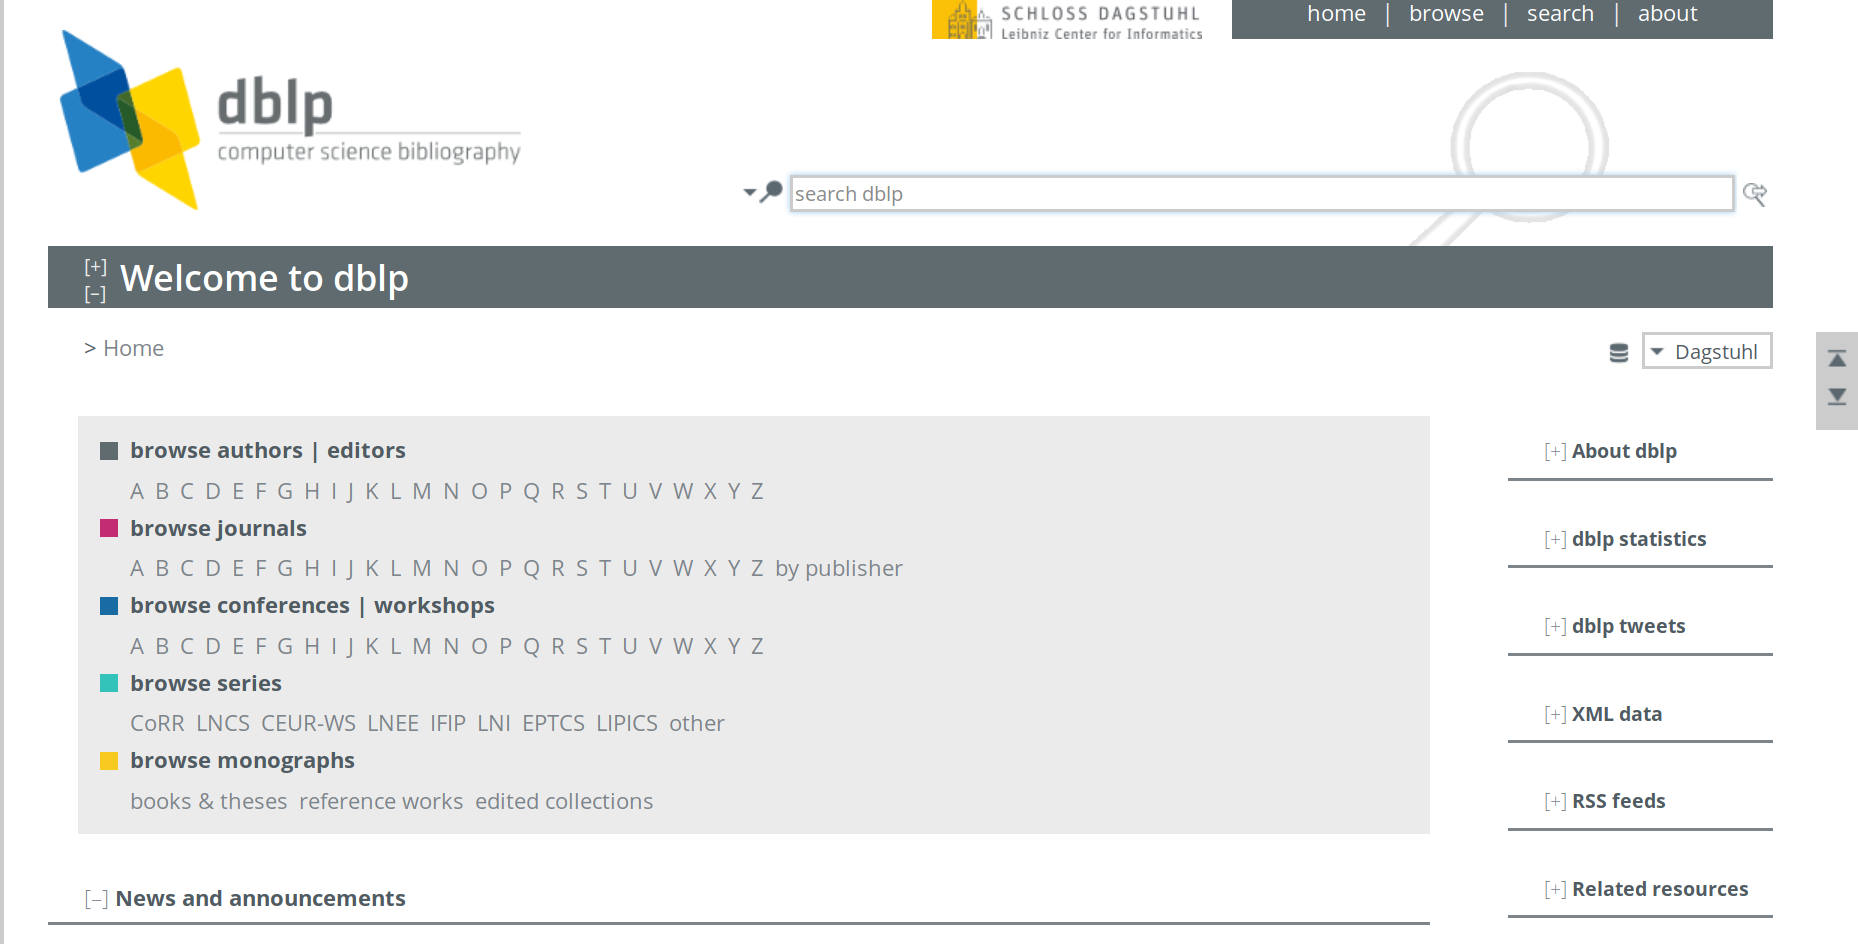
\includegraphics[width=\textwidth,height=0.6\textheight,keepaspectratio]{img/dblp_main.png}
      \end{center}
    \end{figure}
    \url{https://dblp.org/}
\end{frame}
\note[itemize]{
    \item on-line reference for bibliographic information on CS
    \item free access to high-quality bibliographic meta-data
}

\begin{frame}{\currentname}\linespread{1.5}
    \begin{figure}
      \begin{center}
        
\includegraphics[width=\textwidth,height=0.6\textheight,keepaspectratio]{img/this_paper.eps}
      \end{center}
    \end{figure}
    \url{https://doi.org/10.1145/3197026.3197069}
\end{frame}
\note[itemize]{
    \item here's such a bibliographic item
    \item it is the paper to this talk
    \item also url to the paper
    \item I will put slide at the end again
}

\begin{frame}{\currentname}\linespread{1.5}
    \begin{figure}
      \begin{center}
        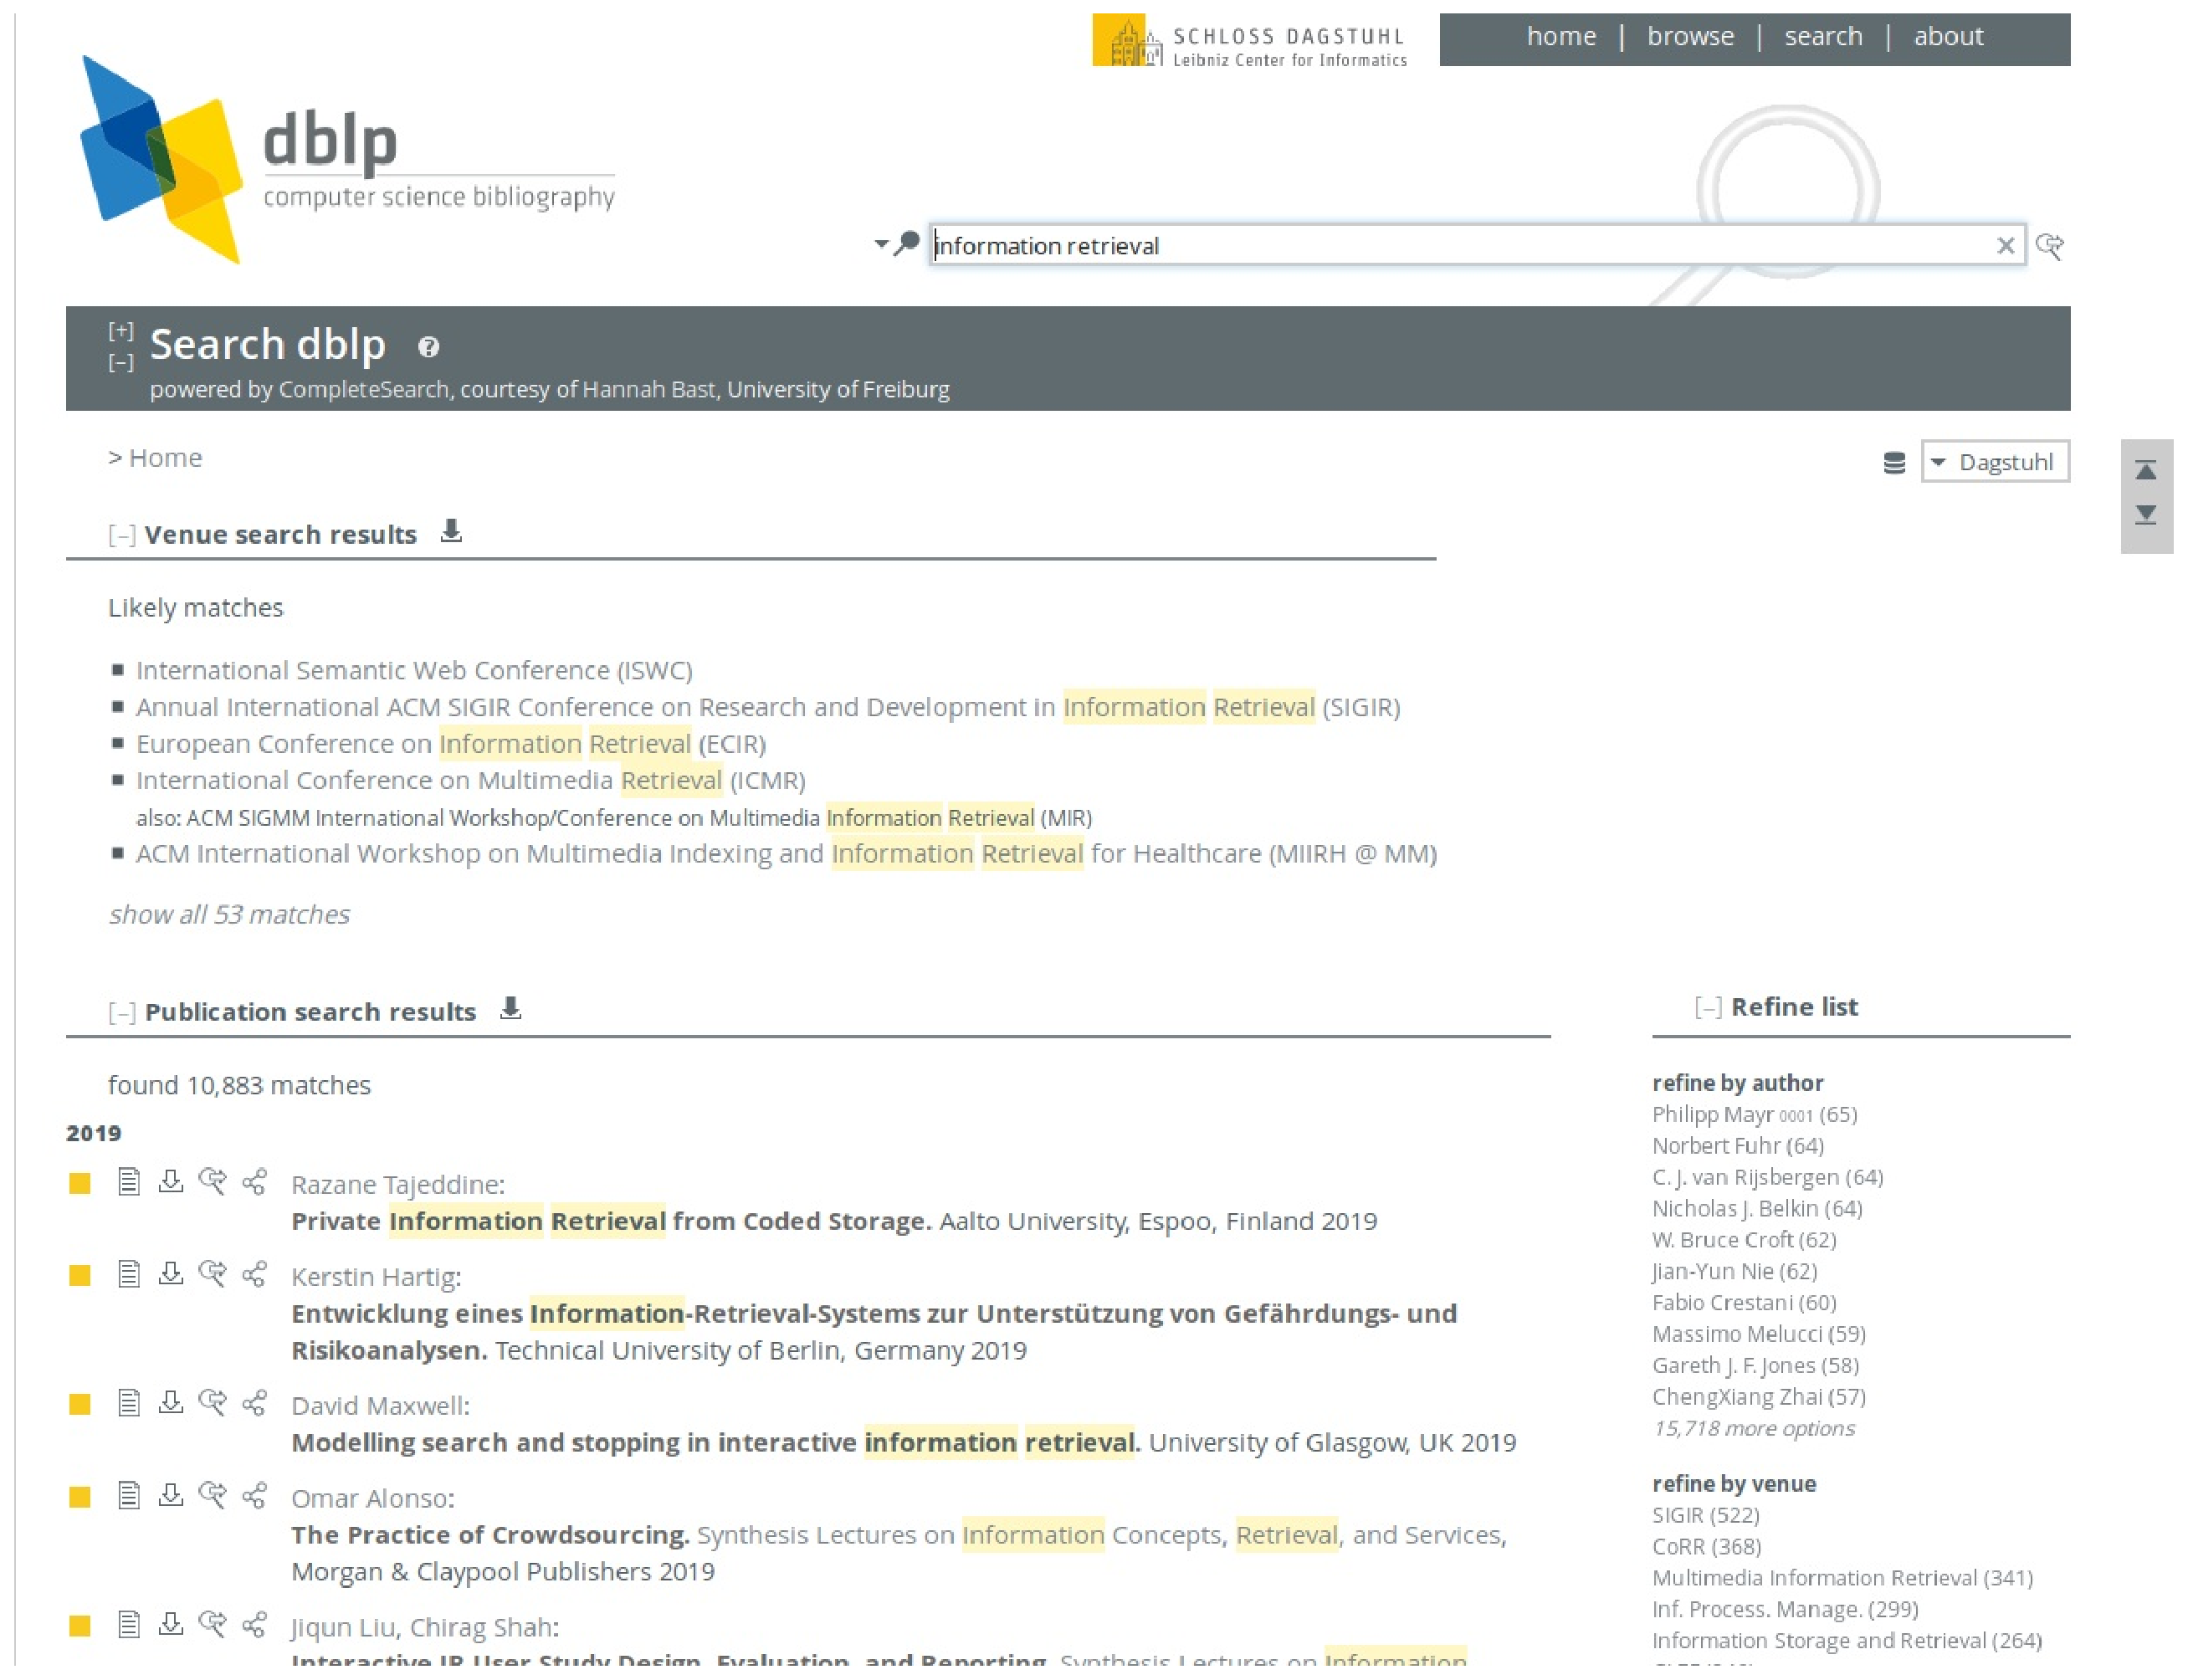
\includegraphics[width=\textwidth,height=0.8\textheight,keepaspectratio]{img/dblp_search.eps}
      \end{center}
    \end{figure}
\end{frame}
\note[itemize]{
    \item keyword-based search possible
    \item results: venues, publications
}

\begin{frame}{\currentname}\linespread{1.5}
    \begin{figure}
      \begin{center}
        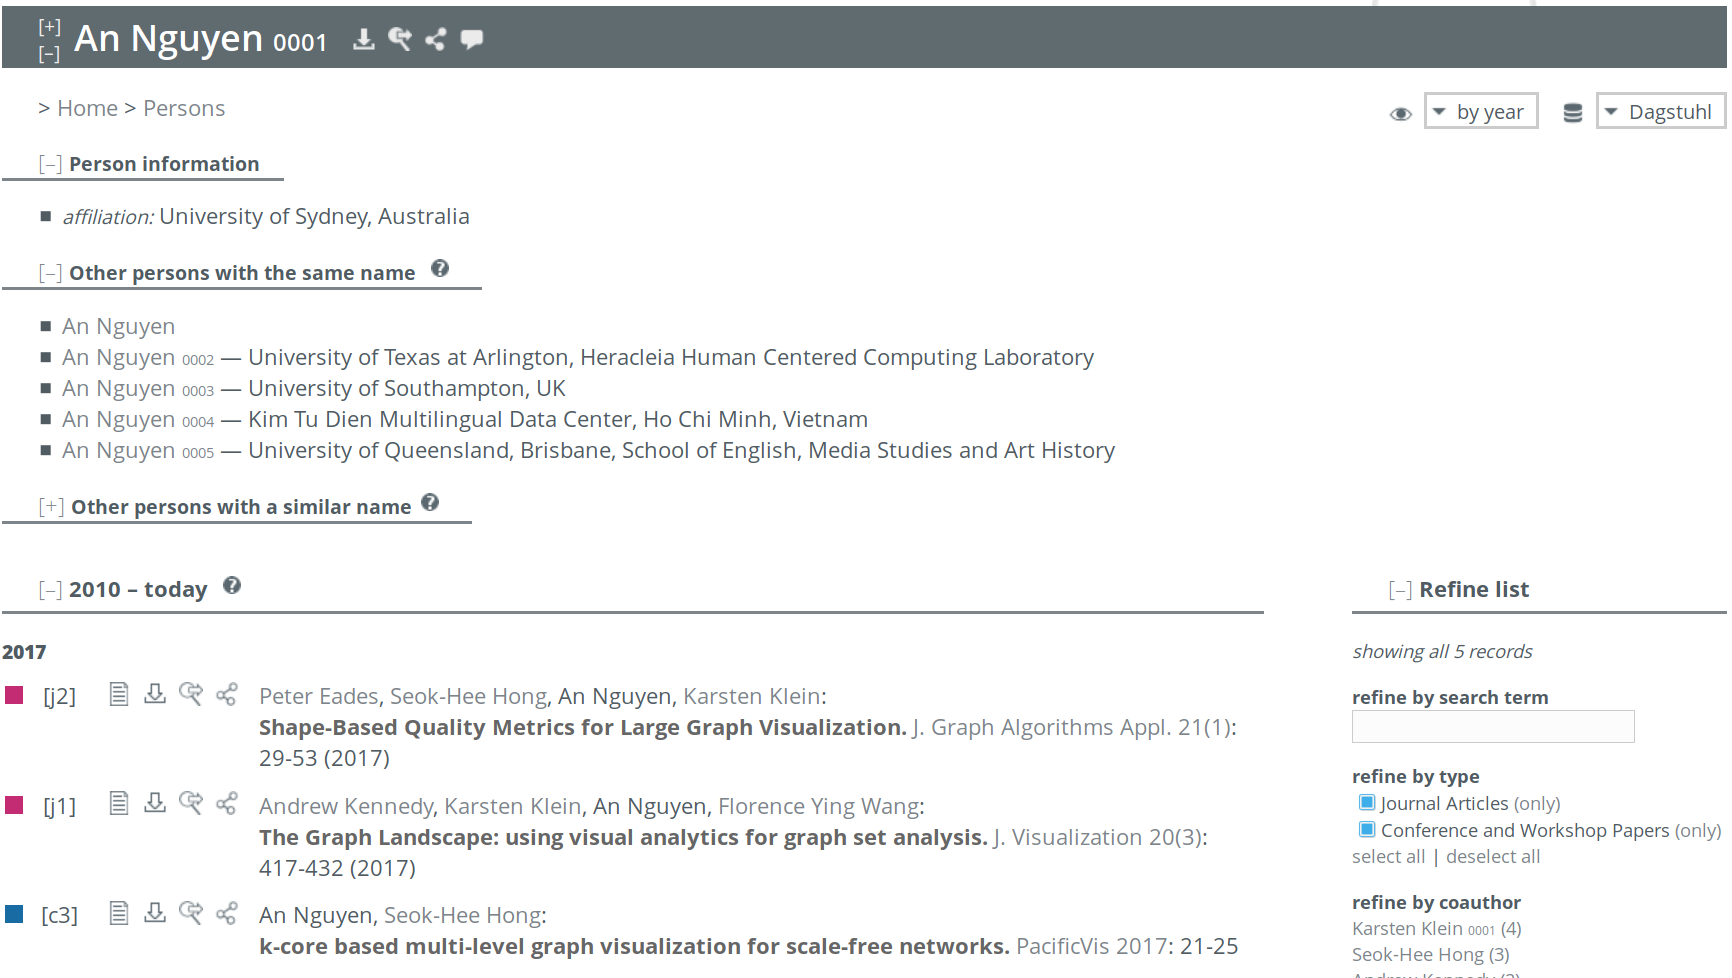
\includegraphics[width=\textwidth,height=0.8\textheight,keepaspectratio]{img/dblp_author_entry.png}
      \end{center}
    \end{figure}
\end{frame}
\note[itemize]{
    \item publications connected with authors
    \item author disambiguation
}

\begin{frame}{\currentname}\linespread{1.5}
    \begin{figure}
      \begin{center}
        
\includegraphics[width=\textwidth,height=0.8\textheight,keepaspectratio]{img/dblp_journal.png}
      \end{center}
    \end{figure}
\end{frame}
\note[itemize]{
    \item browse journals
    \item investigate specific volume of journal
}

\begin{frame}{\currentname}\linespread{1.5}
    \begin{figure}
      \begin{center}
        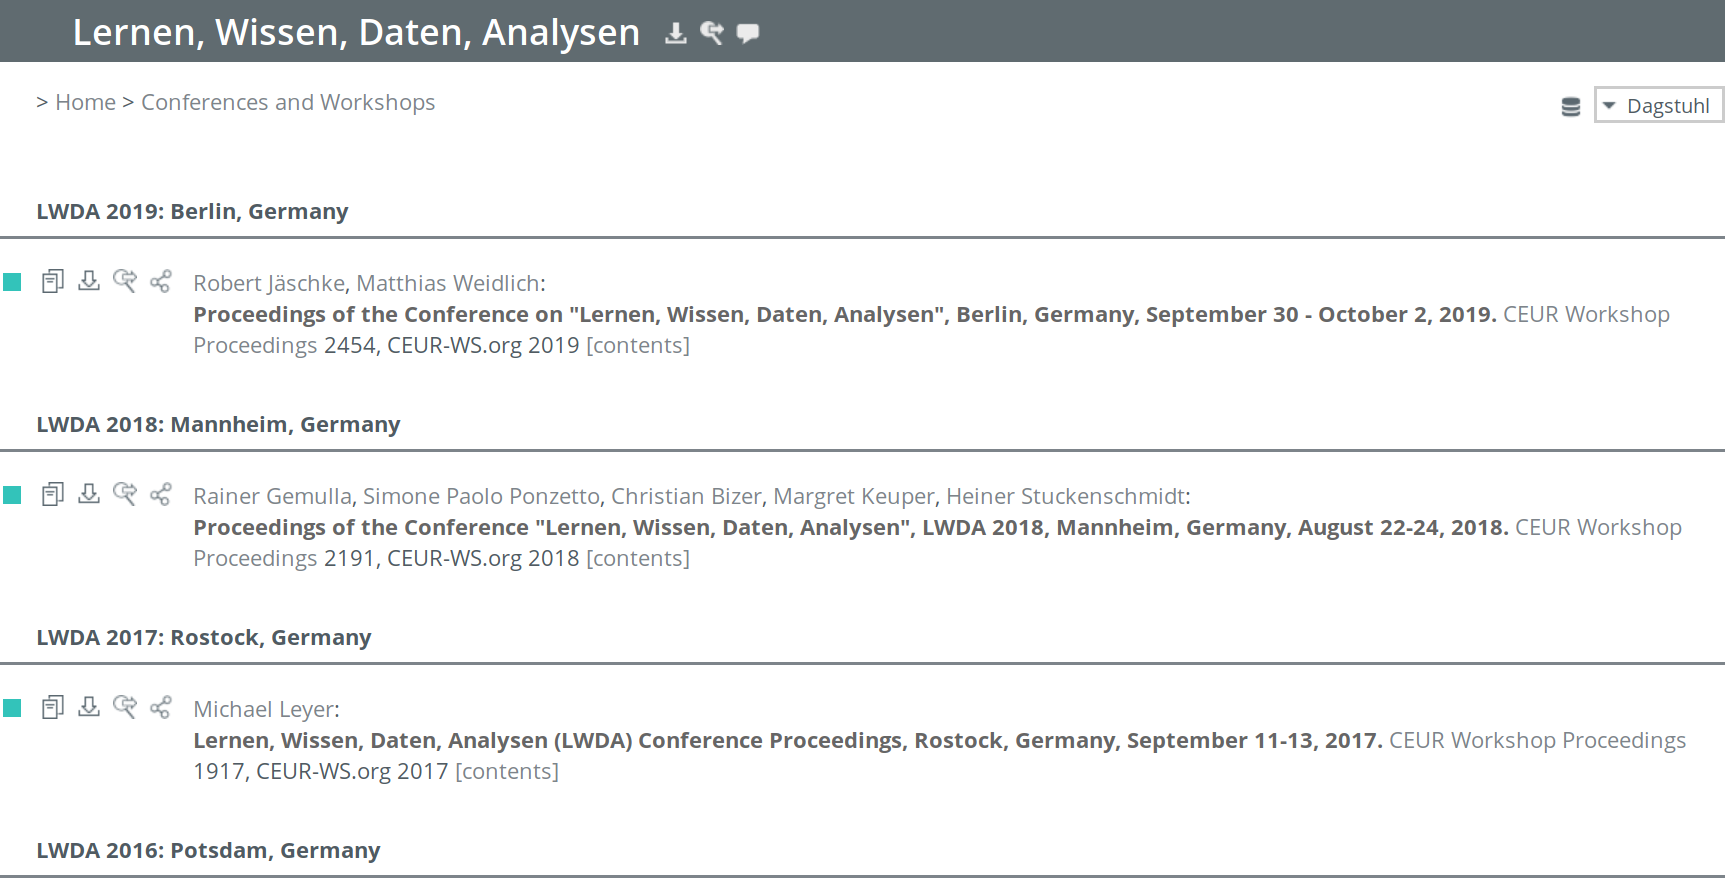
\includegraphics[width=\textwidth,height=0.8\textheight,keepaspectratio]{img/dblp_conference.png}
      \end{center}
    \end{figure}
\end{frame}
\note[itemize]{
    \item browse conference
    \item list of events of which proceedings are present
}

\begin{frame}{\currentname}\linespread{1.5}
    \begin{figure}
      \begin{center}
        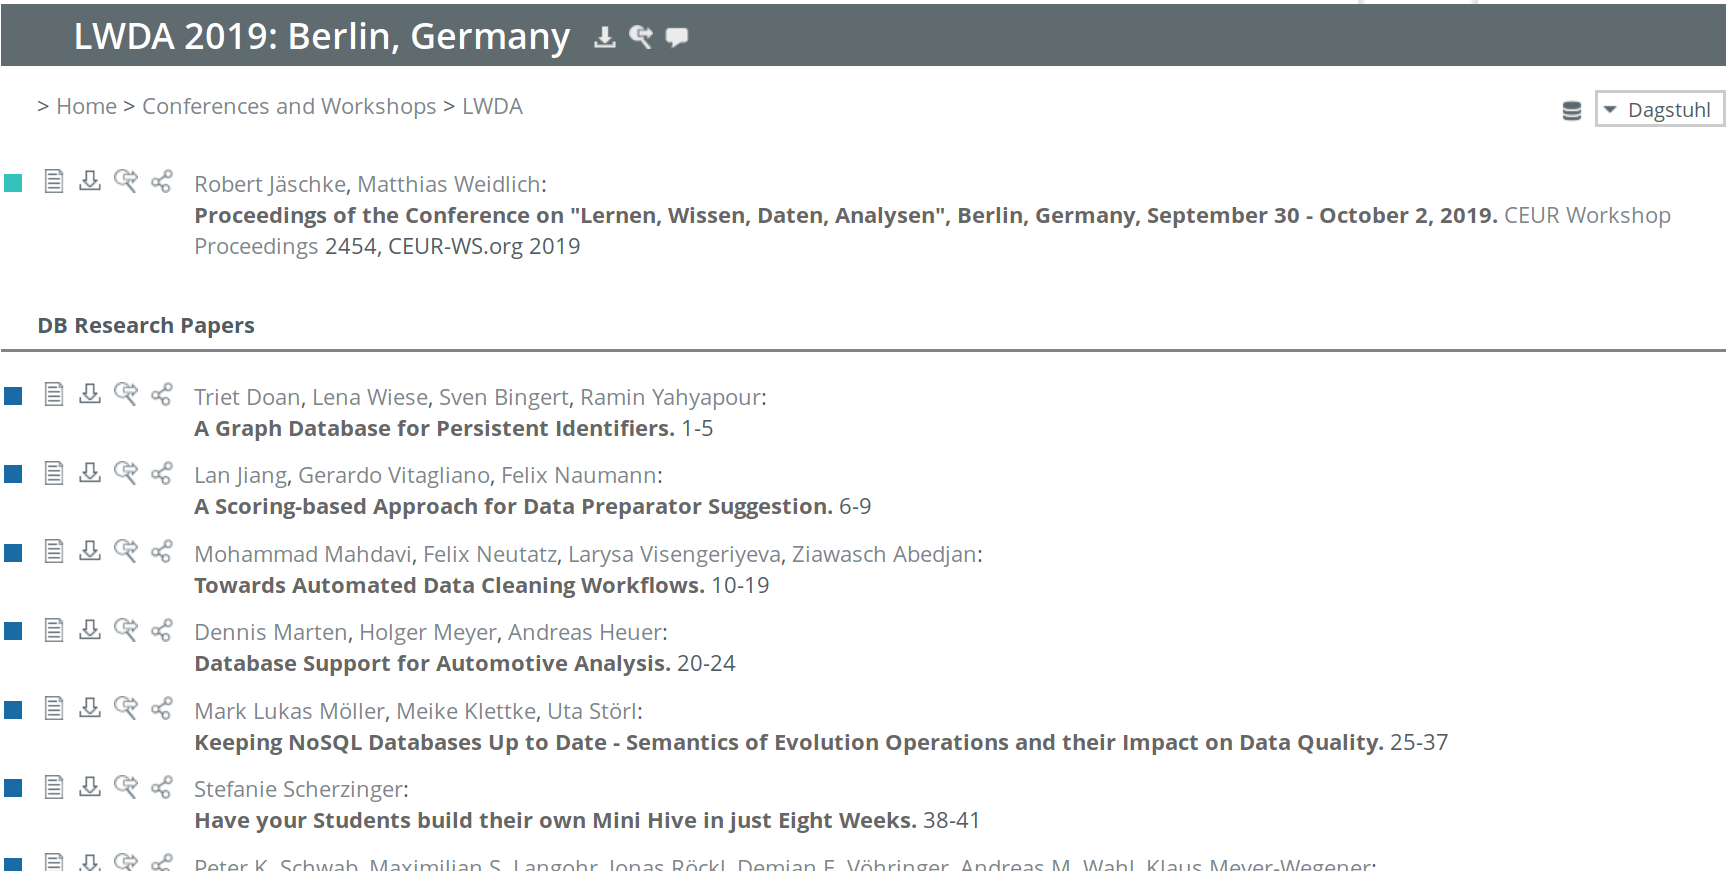
\includegraphics[width=\textwidth,height=0.8\textheight,keepaspectratio]{img/dblp_proceeding.png}
      \end{center}
    \end{figure}
\end{frame}
\note[itemize]{
    \item click on content -- proceeding paper records
}

%------------------------------------------------------------------------------
\subsection{Maintaining the dblp Bibliography}
%------------------------------------------------------------------------------
\begin{frame}{\currentname}\linespread{1.5}

%note: work motivated by current challenges that dblp is facing
% Some statistics on dblp:
%
%   \begin{itemize}
%     \item \textgreater 4.7 million publication records
%     \item originating from \( \approx \)5,700 conferences and \( \approx \)1,600 journals
%   \end{itemize}

\begin{figure}
  \begin{center}
    
\includegraphics[width=\textwidth,height=0.6\textheight,keepaspectratio]{img/documents.pdf}
  \end{center}
\end{figure}
\centering
4.7m
\end{frame}
\note[itemize]{
    \item what does it mean to maintain the dblp?
    \item 4.7 million records in total
    \item in the following I will show you some statistics
    \item related to the research motivation
}

\begin{frame}{\currentname}{}\linespread{1.5}
  %note: distribution of publication types shows that more than half of all records in dblp originate from conference and workshops proceedings
  \begin{figure}
    \begin{center}
      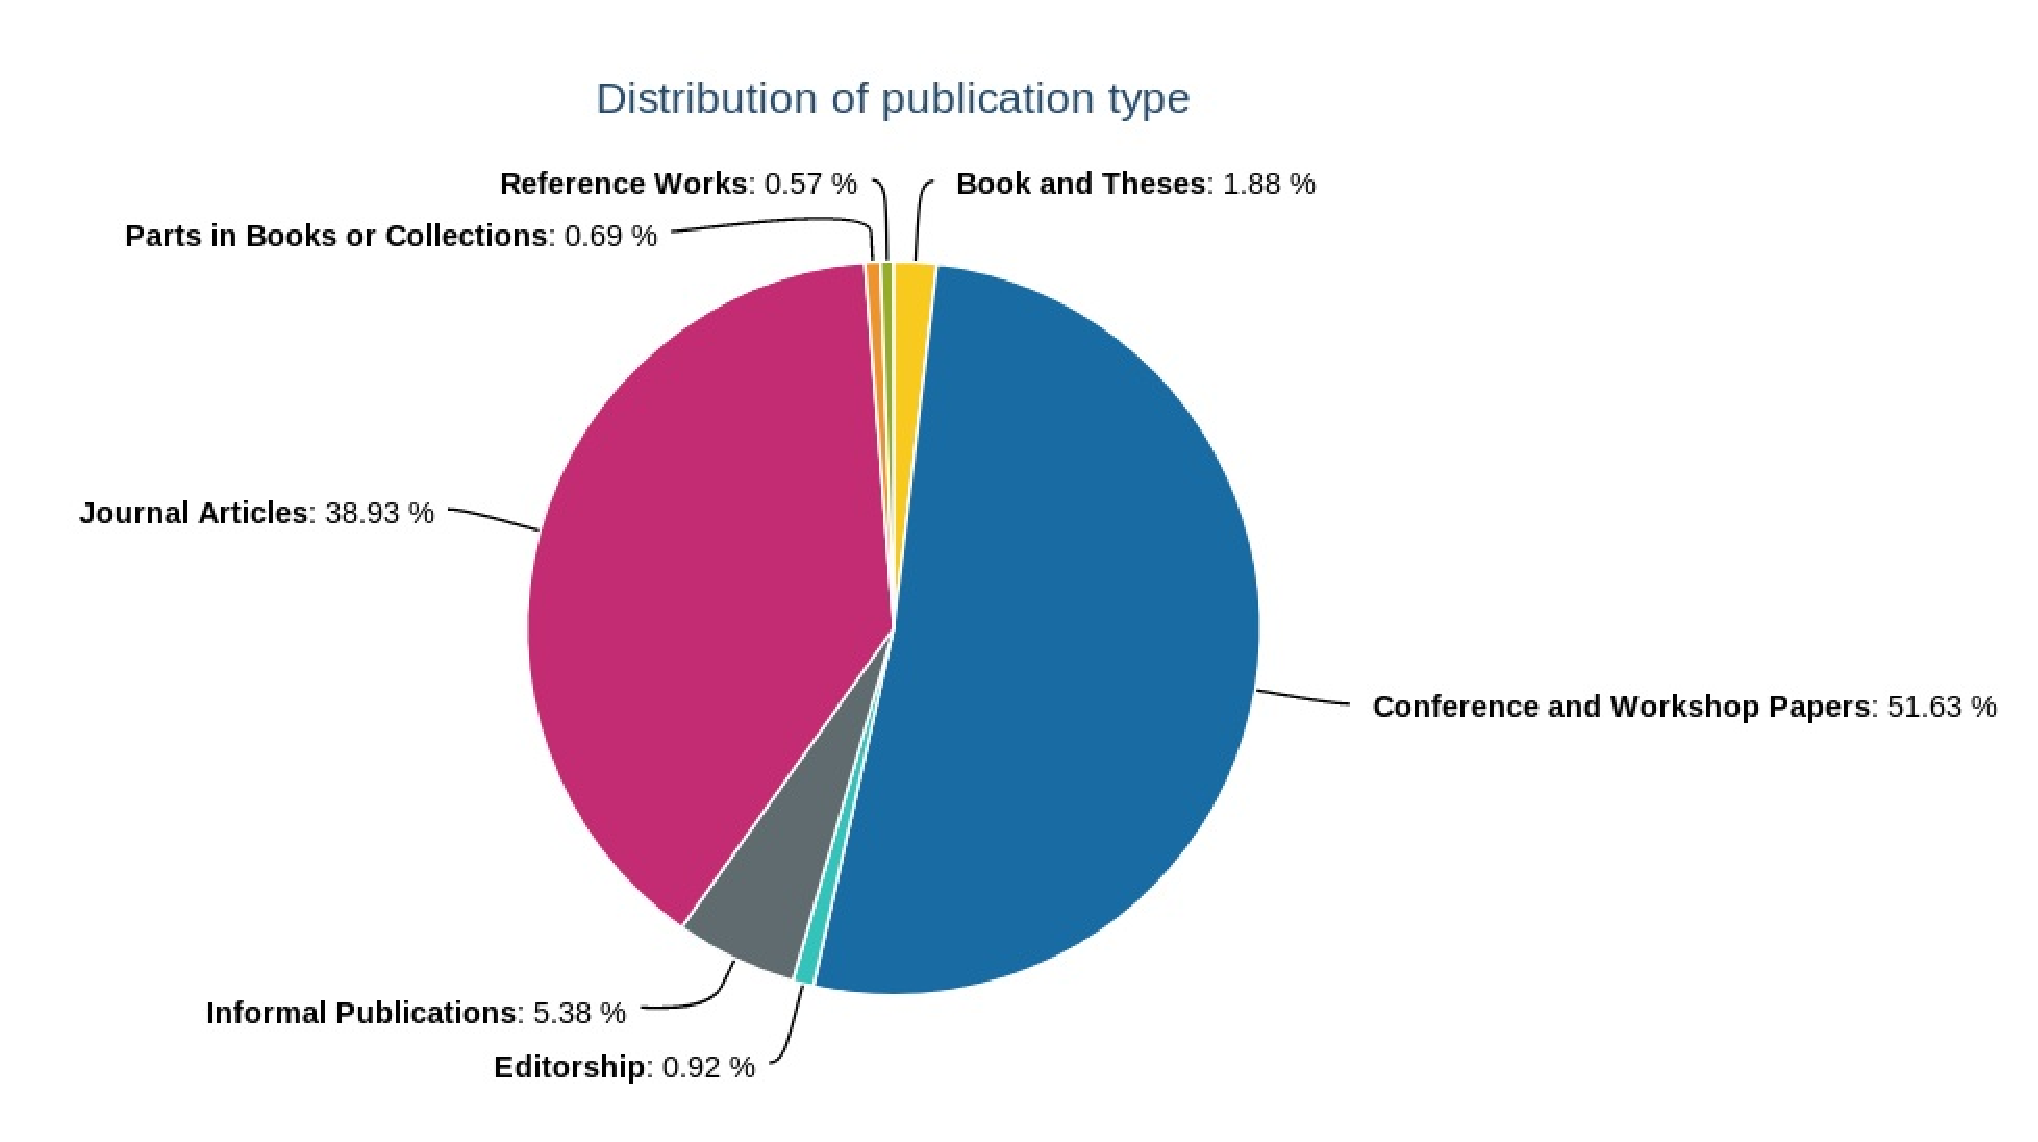
\includegraphics[width=\textwidth,height=0.6\textheight,keepaspectratio]{img/distributionofpublicationtype_2019.eps}
    \end{center}
  \end{figure}
\end{frame}
\note[itemize]{
    \item conferences contribute to the lion's share of research
    \item more than half of all records originate from conference or workshop proceedings
    \item another large share are journal articles
    \item other types of publication are neglectible
}

\begin{frame}{\currentname}{}\linespread{1.5}
  %note: also, the number of new entries to the dblp database per year is constantly growing; here: conference publication entries per year in the last few years always more than 150,000
  New entries to the database per year: conference and workshop papers
  \begin{figure}
    \begin{center}
      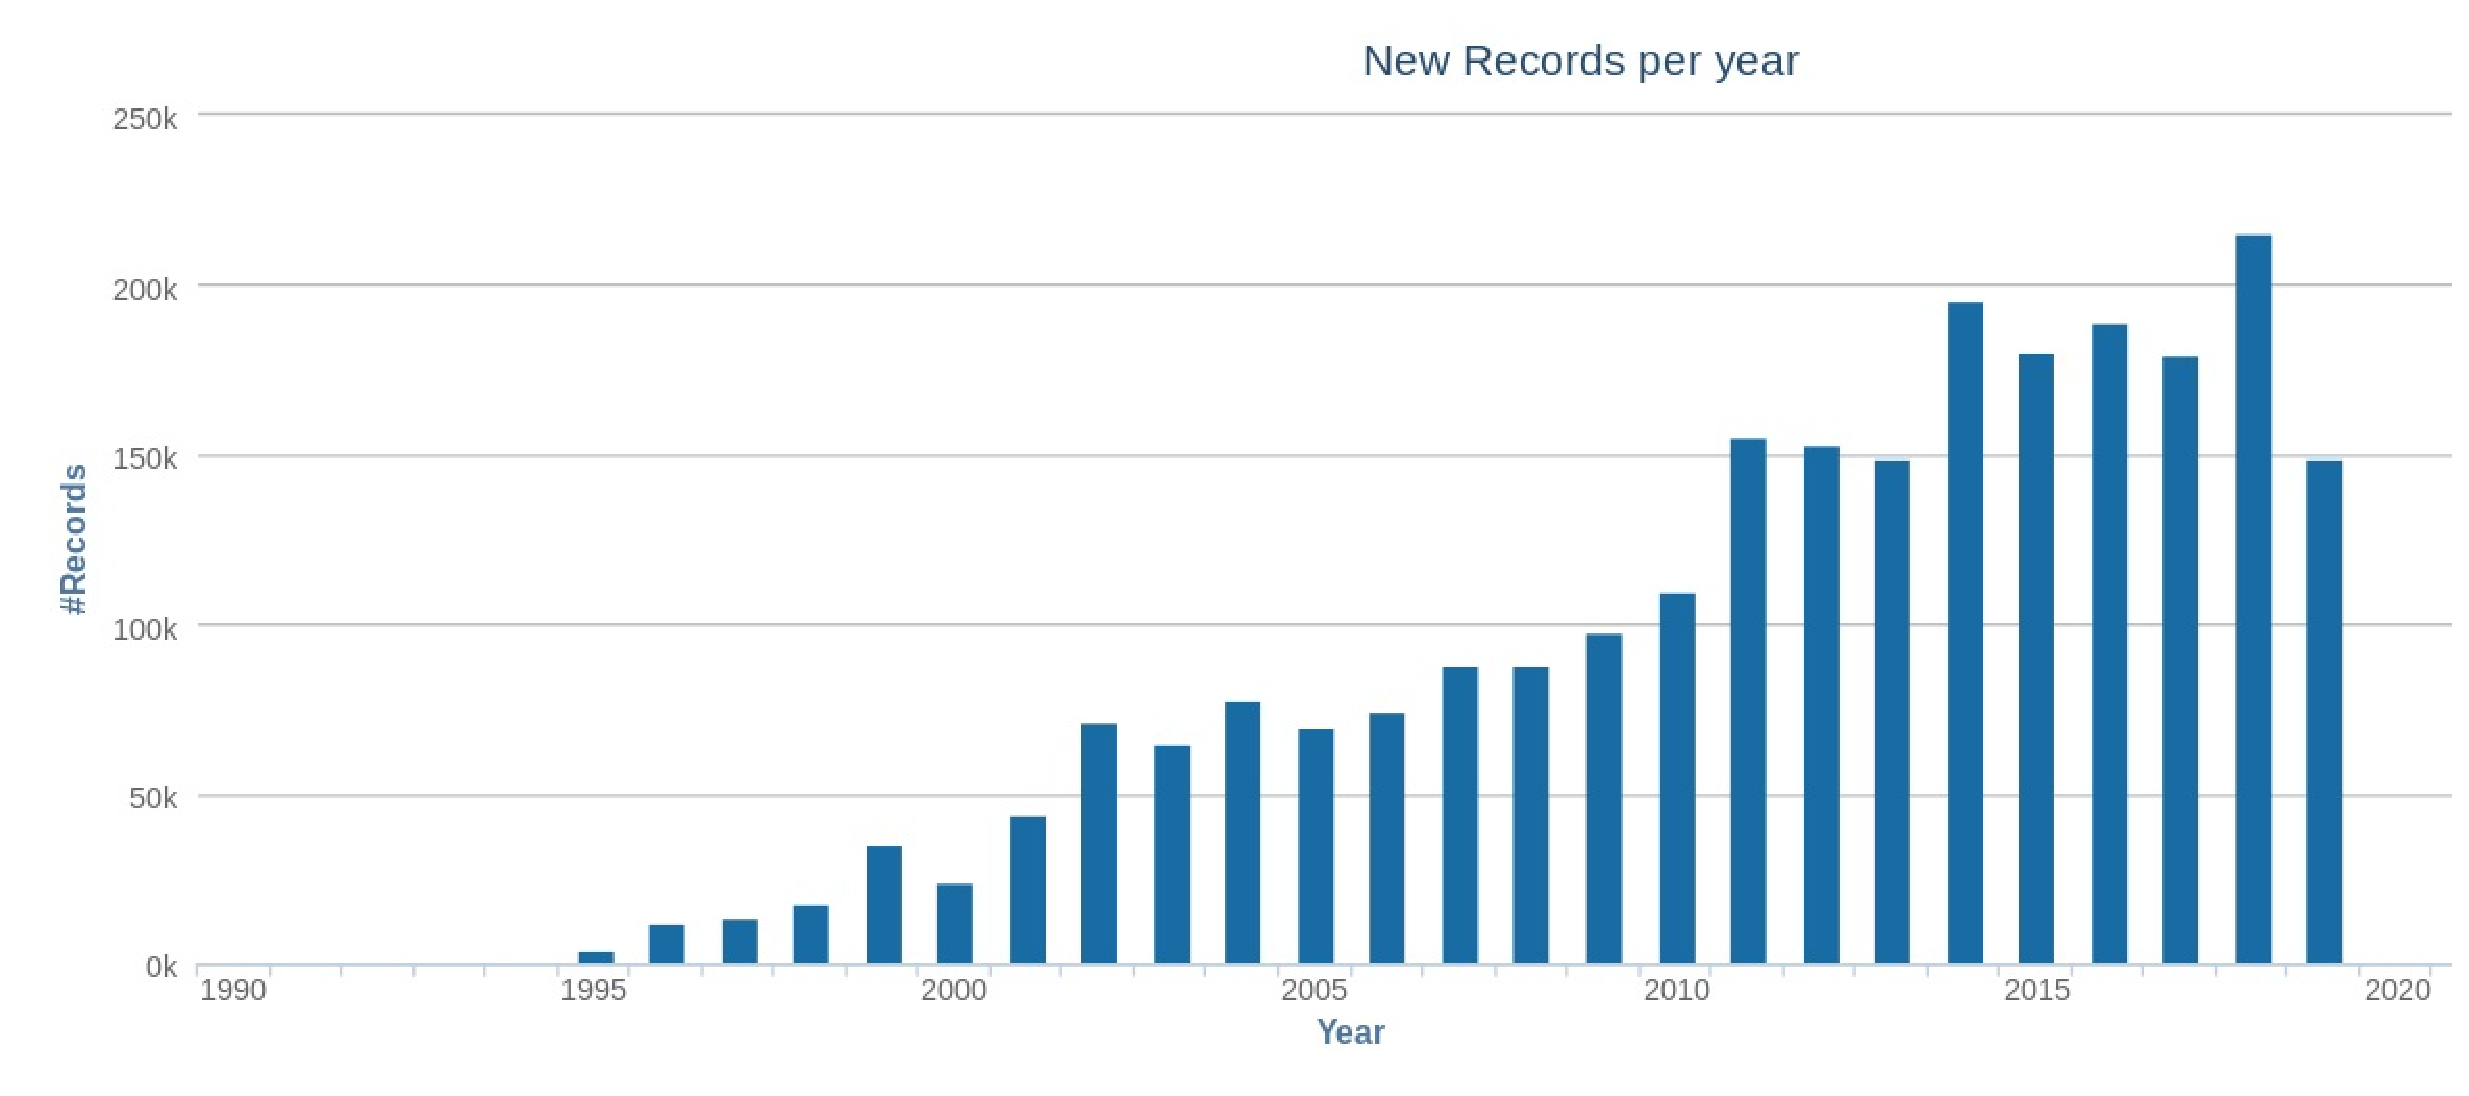
\includegraphics[width=\textwidth,height=0.8\textheight,keepaspectratio]{img/confrecordsperyear_2019.eps}
    \end{center}
  \end{figure}
\end{frame}
\note[itemize]{
    \item focusing on conference and workshop papers here
    \item past years: around 200k new entries per year
    \item i.e. 4k per week
    \item entries are bundled since only complete proceedings are added
    \item still a lot of work (ca. 100-200 proceedings per month)
}

\begin{frame}{\currentname}{}\linespread{1.5}
  %note: these numbers show that there is a massive workload, and that dblp needs efficient monitoring at all stages of their workflow to keep up the high quality of their service
  %the sources of dblp are in particular: ...
  \begin{figure}
    \begin{center}
      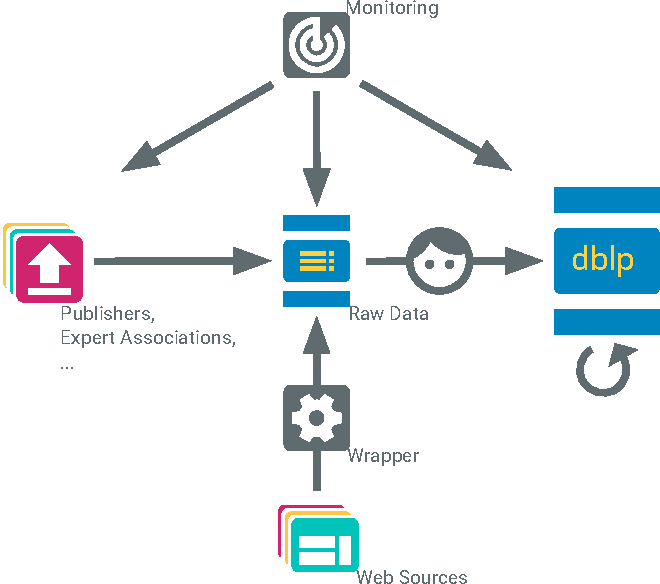
\includegraphics[width=\textwidth,height=0.8\textheight,keepaspectratio]{img/dblp-sources.pdf}
    \end{center}
  \end{figure}
\end{frame}
\note[itemize]{
    \item dblp workflow
    \item sources for raw data: provided, or harvested/scraped
    \item manual work involved to put raw data into system
    \item quality control!
    \item all steps have to be monitored
    \item this is where this research fits in
}

%------------------------------------------------------------------------------
\subsection{Keeping the Archive up to Date -- Obstacles}
%------------------------------------------------------------------------------
\begin{frame}{\currentname}{}\linespread{1.5}
  \note[item]<1->{main challenges}
  \note[item]<1>{time}
  \note[item]<2>{budget}
  \note[item]<3>{personnel}
  \note[item]<4>{irregular schedules, will explain in a minute in more detail}
  \note[item]<5>{not all records are equally important}
  \begin{itemize}
    \item<1->limited resources
    \item<4->conference proceedings
    \item<5>implicit relevance decisions
  \end{itemize}

  \includegraphics<1-3>[width=80pt,height=80pt,keepaspectratio]{img/time.eps}%
  \includegraphics<2-3>[width=80pt,height=80pt,keepaspectratio]{img/budget.eps}%
  \includegraphics<3>[width=80pt,height=80pt,keepaspectratio]{img/personnel.eps}%
  \centering\includegraphics<4>[width=100pt,height=100pt,keepaspectratio]{img/irregular_schedule.eps}%
  \centering\includegraphics<5>[width=80pt,height=80pt,keepaspectratio]{img/relevance_decision.eps}%
\end{frame}

%------------------------------------------------------------------------------
\section{Research Question}
%------------------------------------------------------------------------------

\begin{frame}{\currentname}{}\linespread{1.5}
  \bigskip

  How can we find a prioritization mechanism for conference series with regard to their expected urgency for the data acquisition process at a given point in time?

  \bigskip

  \( \rightarrow \)  Ranking problem: have the conferences for which an update is expected next ranked highest
\end{frame}

%------------------------------------------------------------------------------
\section{Method}
%------------------------------------------------------------------------------

\begin{frame}{\currentname}\linespread{1.5}
  In fact, we are trying to \textit{model} the relevance decisions of our archive curators.

  \centering
  
\includegraphics[width=100pt,height=100pt,keepaspectratio]{img/relevance_decision.eps}
  
\includegraphics[width=100pt,height=100pt,keepaspectratio]{img/prioritization.eps}
\end{frame}
\note[itemize]{
    \item factors loosely based on information quality / dblp quality criteria
    \item see dblp quality criteria: ``The set of authors should be international.''
}

\begin{frame}{\currentname}\linespread{1.5}
    Basis: temporal patterns
    \begin{itemize}
        \item base calculations on patterns from historical data
        \item use relation between past event dates and dates of entry to dblp
    \end{itemize}
    
\includegraphics[width=100pt,height=100pt,keepaspectratio]{img/temporal_pattern.eps}%
    
\includegraphics[width=100pt,height=100pt,keepaspectratio]{img/entry_date.eps}%
\end{frame}
\note[itemize]{
    \item publication date not available
    \item use entry date as approximation of publication date
    \item coming back to irregularities: example
}

% %%test slide for tikz
% \begin{frame}
%
%   \begin{tikzpicture}[scale=3]
%
%     \draw[step=.5cm,gray,very thin] (-1.4,-1.4) grid (1.4,1.4);
%
%     \filldraw [gray]  (0,0) circle (2pt)
%                       (1,1) circle (2pt)
%                       (2,1) circle (2pt)
%                       (2,0) circle (2pt);
%     \draw (0,0) .. controls (1,1) .. (2,0);
%
%     \draw (-1.5,0) -- (1.5,0);
%     \draw (0,-1.5) -- (0,1.5);
%
%     \draw[loosely dotted] (0,0) circle (1cm);
%     \draw (0,0) rectangle (0.5,0.5);
%     \draw (-0.5,-0.5) rectangle (-1,-1);
%
%     \node at ( 0,2) [circle,draw] {a};
%     \node at ( 0,1) [circle,draw] {e};
%     \node at ( 0,0) [circle,draw] {i};
%     \node at ( 1,1) [rectangle,draw] {o};
%     \node at (-1,1) [rectangle,draw] {u};
%
%   \end{tikzpicture}
% \end{frame}
% %%end test slide for tikz

% \makeatletter
% %
%     % This way you can define your own conditions, for example, you
%     % could make something as `full moon', `even week', `odd week',
%     % et cetera. In principle. The math in TeX could be hard.
%     \pgfkeys{/pgf/calendar/start of year/.code={%
%         \ifnum\pgfcalendarifdateday=1\relax%
%             \ifnum\pgfcalendarifdatemonth=1\relax\pgfcalendarmatchestrue\fi%
%         \fi%
%     }}%
% %
%     % Define our own style
%     \tikzstyle{week list sunday}=[
%         % Note that we cannot extend from week list,
%         % the execute before day scope is cumulative
%         execute before day scope={%
%                \ifdate{day of month=1}{\ifdate{equals=\pgfcalendarbeginiso}{}{
%                % On first of month, except when first date in calendar.
%                    \pgfmathsetlength{\pgf@y}{\tikz@lib@cal@month@yshift}%
%                    \pgftransformyshift{-\pgf@y}
%                }}{}%
%         },
%         execute at begin day scope={%
%             % Because for TikZ Monday is 0 and Sunday is 6,
%             % we can't directly use \pgfcalendercurrentweekday,
%             % but instead we define \c@pgf@counta (basically) as:
%             % (\pgfcalendercurrentweekday + 1) % 7
%             \pgfmathsetlength\pgf@x{\tikz@lib@cal@xshift}%
%             \ifnum\pgfcalendarcurrentweekday=6
%                 \c@pgf@counta=0
%             \else
%                 \c@pgf@counta=\pgfcalendarcurrentweekday
%                 \advance\c@pgf@counta by 1
%             \fi
%             \pgf@x=\c@pgf@counta\pgf@x
%             % Shift to the right position for the day.
%             \pgftransformxshift{\pgf@x}
%         },
%         execute after day scope={
%             % Week is done, shift to the next line.
%             \ifdate{Saturday}{
%                 \pgfmathsetlength{\pgf@y}{\tikz@lib@cal@yshift}%
%                 \pgftransformyshift{-\pgf@y}
%             }{}%
%         },
%         % This should be defined, glancing from the source code.
%         tikz@lib@cal@width=7
%     ]
% %
%     % New style for drawing the year, it is always drawn
%     % for January
%     \tikzstyle{year label left}=[
%         execute before day scope={
%             \ifdate{start of year}{
%                 \drawyear
%             }{}
%         },
%         % Right align
%         every year/.append style={
%             anchor=east,
%         }
%     ]
% %
%     % Style to force giving a month a year label.
%     \tikzset{draw year/.style={
%         execute before day scope={
%             \ifdate{day of month=1}{\drawyear}{}
%         }
%     }}
% %
%     % This actually draws the year.
%     \newcommand{\drawyear}{
%         \pgfmathsetlength{\pgf@x}{\tikz@lib@cal@xshift}%
%         \pgftransformxshift{-\pgf@x}
%         % \tikzyearcode is defined by default
%         \tikzyearcode
%         \pgfmathsetlength{\pgf@x}{\tikz@lib@cal@xshift}%
%         \pgftransformxshift{\pgf@x}
%     }
% %
%     \makeatother

\begin{frame}
    \note[item]<1>{2014: conf in june, enter proceeding in september}
    \note[item]<2>{2015: basically same pattern}
    \note[item]<3>{2016: conf a month later, but proceeding added sooner}
    \note[item]<4>{2017: conf again in june, proceeding added later}
    \note[item]<5>{2018: pattern as few years before}
    \only<1>{2014}
    \only<2>{2015}
    \only<3>{2016}
    \only<4>{2017}
    \only<5>{2018}
    \begin{center}
        % \begin{tikzpicture}[scale=0.6, every calendar/.style={
        %     month label above centered,
        %       month text={\textit{\%mt}},
        %       year label left,
        %   }]
        \begin{tikzpicture}[scale=0.6]

          \scriptsize
          \foreach \i in {1,...,12}
          {
            \pgfmathtruncatemacro{\y}{(\i - 1) / 4};
            \pgfmathtruncatemacro{\x}{\i - 4 * \y};
            \only<1>\calendar (cal) [dates=2014-\i-01 to 2014-\i-last, month label above centered, week list, day xshift=1.9em] at (4*\x,-4*\y);
            \only<2>\calendar (cal) [dates=2015-\i-01 to 2015-\i-last, month label above centered, week list] at (4*\x,-4*\y);
            \only<3>\calendar (cal) [dates=2016-\i-01 to 2016-\i-last, month label above centered, week list] at (4*\x,-4*\y);
            \only<4>\calendar (cal) [dates=2017-\i-01 to 2017-\i-last, month label above centered, week list] at (4*\x,-4*\y);
            \only<5>\calendar (cal) [dates=2018-\i-01 to 2018-\i-last, month label above centered, week list] at (4*\x,-4*\y);
          }

          \only<1>{\draw[red,ultra thick]($(cal-2014-06-17.south east) + (-1.2mm,1.2mm)$) rectangle ($(cal-2014-06-17.north west) + (1.2mm,-1.2mm)$){};}
          \only<1>{\draw[blue,ultra thick]($(cal-2014-09-25.south east) + (-1.2mm,1.2mm)$) rectangle ($(cal-2014-09-25.north west) + (1.2mm,-1.2mm)$){};}

          \only<2>{\draw[red,ultra thick]($(cal-2015-06-14.south east) + (-1.2mm,1.2mm)$) rectangle ($(cal-2015-06-14.north west) + (1.2mm,-1.2mm)$){};}
          \only<2>{\draw[blue,ultra thick]($(cal-2015-09-12.south east) + (-1.2mm,1.2mm)$) rectangle ($(cal-2015-09-12.north west) + (1.2mm,-1.2mm)$){};}

          \only<3>{\draw[red,ultra thick]($(cal-2016-07-26.south east) + (-1.2mm,1.2mm)$) rectangle ($(cal-2016-07-26.north west) + (1.2mm,-1.2mm)$){};}
          \only<3>{\draw[blue,ultra thick]($(cal-2016-08-22.south east) + (-1.2mm,1.2mm)$) rectangle ($(cal-2016-08-22.north west) + (1.2mm,-1.2mm)$){};}

          \only<4>{\draw[red,ultra thick]($(cal-2017-06-12.south east) + (-1.2mm,1.2mm)$) rectangle ($(cal-2017-06-12.north west) + (1.2mm,-1.2mm)$){};}
          \only<4>{\draw[blue,ultra thick]($(cal-2017-10-11.south east) + (-1.2mm,1.2mm)$) rectangle ($(cal-2017-10-11.north west) + (1.2mm,-1.2mm)$){};}

          \only<5>{\draw[red,ultra thick]($(cal-2018-06-25.south east) + (-1.2mm,1.2mm)$) rectangle ($(cal-2018-06-25.north west) + (1.2mm,-1.2mm)$){};}
          \only<5>{\draw[blue,ultra thick]($(cal-2018-09-15.south east) + (-1.2mm,1.2mm)$) rectangle ($(cal-2018-09-15.north west) + (1.2mm,-1.2mm)$){};}

          %Legende?
          % \draw[blue,ultra thick] (0,0) rectangle +(1.2mm,-1.2mm) [label=event date] {};
          % \draw[red,ultra thick] (0,0) rectangle +(1.2mm,-1.2mm) [label=entry date]{};

        %shapes examples:
        % \node [draw,regular polygon,regular polygon sides=3] {};
        % \node [draw,cloud] {};
        % \node [fill=yellow,draw,star] {};
        \end{tikzpicture}
    \end{center}
\end{frame}

\begin{frame}{\currentname}\linespread{1.5}
\begin{itemize}
  \item Example conference:
  \begin{itemize}
    \item interval: 1 year
    \item usual month: June
    \item usual delay: 3 months
  \end{itemize}
  \( \rightarrow \) expected: September 2019
  \item 180 other conferences also due in September
  \item base scoring: delay between expected and current date
\end{itemize}
\end{frame}
\note[itemize]{
    \item use median or mode statistics to get these "usual" patterns
}

\begin{frame}{\currentname}\linespread{1.5}
\note[item]<1>{these are the factors we have defined that might influence the prioritization}
\note[item]<1>{and the datasets or how we operationalized the factors}
\note[item]<2>{2 sources for conference ratings: CORE and the one cited here}
\note[item]<3-4>{MAG matched with dblp records where possible}
\note[item]<5-6>{activity in terms of last appearance in dblp in relation to regular interval}
\note[item]<7-8>{internationality in terms of a) venue countries, and b) author affiliations}
\note[item]<9-10>{prominence reflects the share of works in dblp from specific authors}
\note[item]<9-10>{reasoning: proceedings with papers from a lot of prominent authors (for dblp) should be treated with priority}
\note[item]<11-12>{size in terms of average number of papers}
\note[item]<13-14>{log refers to so-called struggling-sessions, where we have signals that users searched for some item without success}
  % \setbeamercovered{transparent}
  \only<1->{Ranking factors and data sets:}
  \begin{itemize}
    \item<1-> conference rating\only<2->{: CORE; Martins et al. \footfullcite{Martins:2009:AssessQualityOfConferences}}
    \item<3-> citation counts\only<4->{: Microsoft Academic Graph (MAG)}
    \item<5-> activity indicator\only<6->{: dblp data}
    \item<7-> internationality\only<8->{: dblp data}
    \item<9-> author prominence\only<10->{: dblp data}
    \item<11-> conference size\only<12->{: dblp data}
    \item<13-> log\only<14->{: dblp data}
  \end{itemize}
\end{frame}

%------------------------------------------------------------------------------
\subsection{Evaluation}
%------------------------------------------------------------------------------
\begin{frame}{\currentname}\linespread{1.5}
  Gold standard:

  \begin{itemize}
    \item human judgments hardly practicable
    \item pseudo-relevance:
    \begin{itemize}
      \item distance in months between current month and month of ingestion into dblp
      \item inverted to give higher values to more recent entries
    \end{itemize}
  \end{itemize}
\end{frame}
%------------------------------------------------------------------------------
\section{Our Results/Contribution}
%------------------------------------------------------------------------------
%------------------------------------------------------------------------------
\subsection{Main Results}
%------------------------------------------------------------------------------

\begin{frame}{\currentname}\linespread{1.5}
    \note[item]<1>{some fluctuation over the year}
    \note[item]<1>{some more than others}
    \note[item]<1>{bold: better than baseline}
    \note[item]<1>{if we average, these 4 factors beat the baseline}
    \note[item]<2>{activity factor with best overall score}
    \note[item]<3>{rating factor consistently above baseline, even if not best on average}
    \note[item]<4>{prominence factor also doing well}
    \note[item]<5>{log factor barely above baseline}
    Overview on \ndcg{}-100 values for each evaluated month with the average.
    \begin{center}
        \resizebox{\textwidth}{!}{
            \begin{tabular}{llllllll|l}
    \toprule
     system & may & jun & jul & aug & sep & oct & nov & avg \\
     \midrule
     base & 0.306 & 0.504 & 0.583 & 0.451 & 0.463 & 0.457 & 0.559 & 0.475 \\
     \tikzmarkin<2>[hl]{a1}active & 0.304 & 0.486 & \textbf{0.655} & \textbf{0.564} & \textbf{0.582} & \textbf{0.556} & \textbf{0.601} & \textbf{0.536}\tikzmarkend{a1}\\
     \tikzmarkin<3>[hl]{b1}rate & \textbf{0.354} & \textbf{0.529} & \textbf{0.615} & \textbf{0.466} & \textbf{0.466} & \textbf{0.518} & \textbf{0.628} & \textbf{0.511}\tikzmarkend{b1}\\
     size & \textbf{0.309} & 0.493 & 0.575 & 0.444 & 0.463 & \textbf{0.461} & \textbf{0.566} & 0.473 \\
     intl & 0.177 & 0.352 & 0.394 & 0.363 & 0.387 & 0.319 & 0.538 & 0.361 \\
     affil & 0.289 & 0.489 & 0.577 & 0.435 & 0.461 & \textbf{0.484} & \textbf{0.563} & 0.471 \\
     cite & 0.305 & 0.495 & 0.574 & 0.443 & 0.460 & 0.456 & 0.552 & 0.469 \\
     \tikzmarkin<4>[hl]{c1}prom & \textbf{0.312} & 0.452 & 0.571 & \textbf{0.481} & \textbf{0.534} & \textbf{0.519} & \textbf{0.591} & \textbf{0.494}\tikzmarkend{c1}\\
     \tikzmarkin<5>[hl]{d1}log & \textbf{0.311} & 0.494 & 0.583 & \textbf{0.476} & \textbf{0.466} & 0.456 & \textbf{0.577} & \textbf{0.480}\tikzmarkend{d1}\\
     \bottomrule
\end{tabular}

        }
    \end{center}
\end{frame}

\begin{frame}{\currentname}\linespread{1.5}
    \note[item]<1>{differences across cut-off levels}
    \note[item]<1>{cut-off 10 or 20 might represent day-to-day work}
    \note[item]<1>{cut-off 100-200 might reflect less frequent, more thorough overview of pending updates}
    \note[item]<1>{also did significance testing here}
    \note[item]<2->{across all cut-off levels, the best performing factors are these three}
    \note[item]<2->{at higher cutoffs, difference to the baseline gains significance}
    Comparison of \ndcg{} values on different cut-offs.
    \begin{center}
        \resizebox{\textwidth}{!}{
            \begin{tabular}{lllll}
     \toprule
     system & \ndcg{10} & \ndcg{20} & \ndcg{100} & \ndcg{200} \\ \midrule
     base & 0.566 & 0.533 & 0.475 & 0.396 \\
     \tikzmarkin<2>[hl]{a2}active (A) & \textbf{0.615} & \textbf{0.588} & \textbf{0.536*} & \textbf{0.517**} \tikzmarkend{a2} \\
     \tikzmarkin<3>[hl]{b2}rate (R) & \textbf{0.567} & \textbf{0.576} & \textbf{0.511**} & \textbf{0.478**} \tikzmarkend{b2} \\
     size & \textbf{0.577} & \textbf{0.540} & 0.473 & \textbf{0.398} \\
     intl & 0.304 & 0.330 & 0.361 & 0.281 \\
     affil & 0.543 & 0.523 & 0.471 & \textbf{0.400} \\
     cite & 0.566 & 0.533 & 0.469 & 0.395 \\
     \tikzmarkin<4>[hl]{c2}prom (P) & 0.535 & \textbf{0.553} & \textbf{0.494} & \textbf{0.485***} \tikzmarkend{c2} \\
     log & 0.560 & 0.528 & \textbf{0.480} & \textbf{0.407*} \\
     \bottomrule
     \multicolumn{5}{c}{${}^{***}=p<0.001$, ${}^{**}=p<0.01$, ${}^{*}=p<0.05 $}
\end{tabular}

        }
    \end{center}
\end{frame}


\begin{frame}{\currentname}\linespread{1.5}
    \note[item]<1>{combine best performing factors}
    \note[item]<1>{combinations with rating perform very well}
    \note[item]<2>{already at low cut-off levels}
    Comparison of \ndcg{} values on different cut-offs for combined factors.
    \begin{center}
        \resizebox{\textwidth}{!}{
            \begin{tabular}{lllll}
    \toprule
    system  & \ndcg{20}      & \ndcg{30}       & \ndcg{100}      & \ndcg{200}    \\ \midrule
    base    & 0.533         & 0.511             & 0.475             & 0.396  \\
    \tikzmarkin<2>[hl]{a3}R $\times$ A      & \textbf{0.628*} & \textbf{0.629***} & \textbf{0.561***} & \textbf{0.547***}\tikzmarkend{a3}\\
    \tikzmarkin<4>[hl]{c3}R $\times$ P         & \textbf{0.582}  & \textbf{0.603**}  & \textbf{0.550**}  & \textbf{0.498***}\tikzmarkend{c3}\\
    \tikzmarkin<3>[hl]{b3}R $\times$ A $\times$ P  & \textbf{0.587}  & \textbf{0.606**}  & \textbf{0.574***} & \textbf{0.542***}\tikzmarkend{b3}\\
    A $\times$ P        & \textbf{0.547}  & \textbf{0.532}    & \textbf{0.529**}  & \textbf{0.509***} \\
    \bottomrule
    \multicolumn{5}{c}{${}^{***}=p<0.001$, ${}^{**}=p<0.01$, ${}^{*}=p<0.05 $}
\end{tabular}

        }
    \end{center}
\end{frame}
%------------------------------------------------------------------------------
\subsection{Interpretation}
%------------------------------------------------------------------------------
\begin{frame}{\currentname}\linespread{1.5}
  Best performing factors in terms of information quality:
  \begin{itemize}
    \item credibility:
    \begin{itemize}
      \item expressed through ratings
    \end{itemize}
    \item currency:
    \begin{itemize}
      \item expressed through activity
    \end{itemize}
    \item popularity:
      \begin{itemize}
        \item expressed through prominence and logs
      \end{itemize}
  \end{itemize}
\end{frame}

%------------------------------------------------------------------------------
\subsection{Limitations}
%------------------------------------------------------------------------------
\begin{frame}{\currentname}\linespread{1.5}
    \begin{itemize}
        \item ratings available for only about 20\% of the data
        \item log data hard to interpret
    \end{itemize}
\end{frame}

%
% \begin{frame}{\currentname}\linespread{1.5}
% \end{frame}
%------------------------------------------------------------------------------
\section*{Summary}
%------------------------------------------------------------------------------
\begin{frame}{\currentname}\linespread{1.5}

  % Keep the summary *very short*.
  \begin{itemize}
    \item
      We can use information quality-related features to rank conferences for data ingestion routines.
      % The \alert{first main message} of your talk in one or two lines.
    \item
    All proposed features outperform the baseline derived from ingestion delays.
      % The \alert{second main message} of your talk in one or two lines.
    % \item
    %   Perhaps a \alert{third message}, but not more than that.
  \end{itemize}

  % The following outlook is optional.
  \vskip0pt plus.5fill
  \begin{itemize}
  \item
    Outlook
    \begin{itemize}
    \item separate workshops
    \item extend approach to journals etc.
    \item Learning to Rank
    \end{itemize}
  \end{itemize}
\end{frame}

%------------------------------------------------------------------------------

\begin{frame}{Discussion}
Thank you for your attention!\\
Feel free to ask any questions now!\bigskip

Contact us:\\
\href{mailto:mandy.neumann@th-koeln.de}{\nolinkurl{mandy.neumann@th-koeln.de}}\\
\href{mailto:michelsc@uni-trier.de}{\nolinkurl{michelsc@uni-trier.de}}\\
\href{mailto:philipp.schaer@th-koeln.de}{\nolinkurl{philipp.schaer@th-koeln.de}}\\
\href{mailto:schenkel@uni-trier.de}{\nolinkurl{schenkel@uni-trier.de}}\bigskip

Visit \url{https://dblp.org}

Read the paper: \url{https://doi.org/10.1145/3197026.3197069}

\end{frame}

%------------------------------------------------------------------------------

\setbeamertemplate{section in toc shaded}[default][100]
  \begin{frame}{Table of contents}
  	\tableofcontents[
      currentsection,
      currentsubsection,
      subsectionstyle=hide
    ]
  \end{frame}

%------------------------------------------------------------------------------

% All of the following is optional and typically not needed.
\appendix
\section<presentation>*{\appendixname}
\subsection<presentation>*{For Further Reading}

% \begin{frame}[allowframebreaks]
%   \frametitle<presentation>{References}
%   \bibliographystyle{amsalpha}
%   \bibliography{main.bib}
% \end{frame}

% \begin{frame}[allowframebreaks]
%   \frametitle<presentation>{For Further Reading}
%
%   \begin{thebibliography}{10}
%
%   \beamertemplatebookbibitems
%   % Start with overview books.
%
%   \bibitem{Author1990}
%     A.~Author.
%     \newblock {\em Handbook of Everything}.
%     \newblock Some Press, 1990.
%
%
%   \beamertemplatearticlebibitems
%   % Followed by interesting articles. Keep the list short.
%
%   \bibitem{Someone2000}
%     S.~Someone.
%     \newblock On this and that.
%     \newblock {\em Journal of This and That}, 2(1):50--100,
%     2000.

%   \end{thebibliography}
% \end{frame}

\end{document}
